\documentclass[12pt, a4paper]{article}

\usepackage{import}
\usepackage{standalone}

\usepackage[top=4cm, right=2cm, bottom=2.7cm, left=2cm]{geometry}

\usepackage{wrapfig}
\usepackage{tabulary}
\usepackage{float}
\usepackage{pifont}
\usepackage{background}
\usepackage{tikz}


\pagestyle{empty}
\setlength{\parindent}{0pt}

\begin{document}
	\begin{minipage}{\textwidth}
		\section{Stokken Sorteren \hfill\small Bron: Bebras}
			
			Help! Robin de robot sorteert boomstammen. Maar we weten niet welk voorschrift hij daarbij volgt.
			
			\begin{figure}[H]
				\centering
				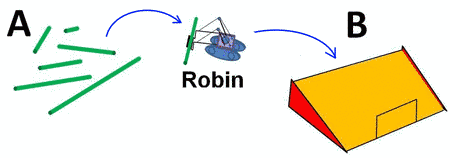
\includegraphics[width=0.7\linewidth]{image1} 
			\end{figure}

			Robin werkt op de volgende manier:
			
			\begin{enumerate}
				\item Bij punt A liggen meerdere boomstammen met verschillende lengte. Robin kiest een boom uit volgens een bepaald voorschrift (zie verder).
				\item Robin legt de boomstam boven aan de rand van een hellend vlak op punt B.
				\item De stam rolt naar beneden tot tegen de andere stammen aan de onderkant van het hellend vlak.
				\item Dit doet Robin net zo lang totdat alle boomstammen op punt B zijn verzameld.
			\end{enumerate}
		
			\begin{minipage}{0.3\linewidth}
				\begin{figure}[H]
					\centering
					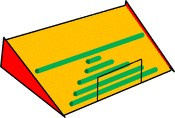
\includegraphics[width=\linewidth]{image2} 
				\end{figure}
			\end{minipage} \hfill
			\begin{minipage}{0.7\linewidth}
				Hiernaast zie je het resultaat. Volgens welk van de volgende voorschriften heeft Robin de boomstammen gekozen?
			\end{minipage} \\
		
			\begin{table}[H]
				\centering
				\begin{tabular}{|c|c|}
					\hline
					\textbf{A} & Neem telkens de op één na kortste boomstam. Is er nog maar één over, neem dan deze. \\
					\textbf{B} & Neem telkens de op één na langste boomstam. Is er nog maar één over, neem dan deze. \\ 
					\textbf{C} & Neem telkens de langste boomstam. \\ 
					\textbf{D} & Neem telkens de kortste boomstam. \\
					\hline 
				\end{tabular}
			\end{table}
	\end{minipage} \\ \\
	
\end{document}	